\documentclass[11pt,a4paper]{scrreprt}

\usepackage{draftwatermark}

\usepackage[left=2.5cm,right=2.5cm,top=2.5cm,bottom=2.5cm]{geometry}
\usepackage{svg}
\usepackage{graphicx}

\usepackage{erewhon}
\usepackage[utf8]{inputenc}
\usepackage[english]{babel}
\usepackage{csquotes}

\usepackage[natbib=true,backend=bibtex]{biblatex}
\addbibresource{refs.bib}

\newcommand{\theauthor}{Gravitalia}
\newcommand{\thetitle}{Turms specification}
\newcommand{\theversion}{0.1.0}

\title{\thetitle}
\author{v\theversion\\\theauthor}
\date{2025-10-24}

% Metadata
\usepackage{hyperref}
\hypersetup{
    pdfauthor={\theauthor},
    pdftitle={\thetitle},
}

% TikZ
\usepackage{tikz}
\usepackage{tikz-uml}
\usepackage{pgfplots}

% Miscellaneous
\usepackage{multicol}
\usepackage{listings}
\usepackage{xcolor} % Driver-independent color extensions for LaTeX
\usepackage[inline,shortlabels]{enumitem}

% Mathematics
\usepackage{amsmath}

% Appendix
\usepackage{appendix}
\usepackage{pdfpages}

\begin{document}

\maketitle
\tableofcontents
\newpage

\section*{Terminology}

\input{terminology}

\chapter{Introduction}
\label{chap:intro}

Gravitalia Turms (\enquote{Turms}) is a point-to-point messaging service. 
Message exchanges are encrypted using multiple layers (\enquote{multi-layer 
encryption,} \enquote{E2EE}). Message storage is encrypted at rest. Turms is 
not yet a peer-to-peer messaging service, as it does not provide indirect 
benefits to other peers\cite{rfc5694}.

\begin{center}
\begin{tikzpicture}
    \umlactor {Peer 1}
    \umlactor [x=6] {Peer 2}
    \umlassoc[arg=Communication, pos=0.5]{Peer 1}{Peer 2}

    \umlusecase[x=3,y=-2,name=discovery]{Discovery server}
    \umlaggreg[style=dashed]{discovery}{Peer 1}
    \umlaggreg[style=dashed]{discovery}{Peer 2}
\end{tikzpicture}
\end{center}

\section{Architecture}
\label{sec:architecture}

Direct communication between clients is often impossible, mainly due to 
firewalls and NAT. Turms' architecture takes these issues into account.

\subsection{Peer discovery}

There are several ways to find peers. Turms implements only two of them:
\begin{enumerate}
    \item SDP sharing
    \item Discovery server
\end{enumerate}

\subsubsection{SDP sharing}

Session Description Protocol (SDP) is an essential component of WebRTC.
% (\ref{subsec:webrtc}).
It allows two peers to connect directly to each other without going through a 
discovery server. SDP contains the codec, source address, and timing 
information for audio and video. During the initial initialization, SDP does 
not contain audio and video codecs. These are renegotiated on the fly when the 
two peers wish to communicate via audio or video. This choice avoids the slight 
overhead of finding the hardware beforehand and then during transmission, when 
it turns out to be unnecessary. SDP also contains information for initiating a 
secure connection (\ref{sec:dlts}).
SDP sharing implies user shares its SDP outside Turms network.
\newpage

Turms SDP MUST contains:
\begin{center}
\begin{tabular}{||c c c||} 
 \hline
 Name & Content & Description \\ [0.5ex] 
 \hline\hline
 v & 0 & SDP version. \\ 
 \hline
 o &  & Session origin. \\ 
 \hline
 s & - & Session name. \\ 
 \hline
 t & 0 0 & Session time. \\ 
 \hline
 a=fingerprint &  & DTLS fingerprint. \\ 
 \hline
 a=group & BUNDLE 0 & Bundled media. \\ 
 \hline
 a=extmap-allow-mixed &  & Mixed RTP extensions. \\ 
 \hline
 m &  & Media description. \\ 
 \hline
 c &  & Connection info. \\ 
 \hline
 a=setup & actpass & DTLS role. \\ 
 \hline
 a=mid & 0 & Media ID. \\ 
 \hline
 a=sendrecv &  & Bidirectional flow. \\ 
 \hline
 a=sctp-port & 5000 & SCTP port. \\ 
 \hline
 a=ice-ufrag &  & ICE username. \\ 
 \hline
 a=ice-pwd &  & ICE password. \\ 
 \hline
 a=candidate & (multiple) & ICE candidates. \\ 
 \hline
 typ host &  & Local candidate. \\ 
 \hline
 typ srflx &  & Reflexive candidate. \\ 
 \hline
 raddr / rport &  & Related address/port. \\ 
 \hline
 a=end-of-candidates &  & End of ICE list. \\ 
 \hline
\end{tabular}
\end{center}

The SDP MUST be passed in JSON format, as:
\begin{center}
    \begin{tikzpicture}
        \umlclass{SDP}{
            + type : String = "offer" | "answer" \\
            + sdp : String
        }{}
    \end{tikzpicture}
\end{center}

%\subsubsection{Discovery server}
%See: \nameref{chap:discovery}

\section{Goals}
\label{sec:goals}

This point-to-point architecture choice ensures the resilience and privacy of 
telecommunications. However, authenticity is more difficult to preserve.

\subsection{Privacy}

The term \enquote{privacy} is semantically rich. It ranges from an individual's 
physical condition to their most fundamental rights \cite{rfc6973}. P2P 
connections avoid some threats. For instance, surveillance is made more tricky; 
uniquely if traffic is encrypted. Since data is stored locally, it relies on 
hardware security measures and only compromises one user in the event of a 
leak. However, it discloses the IP address, this gives an approximate 
geolocation of the peer. To maximize benefits, you SHOULD use onions, but it 
remains complicated.

\subsection{Authenticity}

Authenticity allows the author of a message to be proven. In P2P, authenticity 
is hard to prove. Turms allows individuals to authenticate themselves through 
an Autha instance, or to remain as \enquote{guests.}

\begin{enumerate}
    \item \textbf{Autha instance with discovery server}: discovery server 
validates the decentralized identity, then generates a JWT. During signaling, 
the discovery server acts as a trusted third party. User acquires the ID 
\enquote{user\_id@discovery\_server.tld.} Once the initial connection has been 
established, messages are authenticated by their signature.
    \item \textbf{Autha instance without discovery server}: user generates a 
token that will be sent to the peer, who will verify it using the public key 
provided by the user's Autha instance.
    \item \textbf{As guest}: untrustworthy and inauthentic by nature. Trust is 
acquired through the SDP transmission channel.
\end{enumerate}

\subsection{Integrity}

Integrity ensures that messages has not been altered during transit. This 
component goes hand in hand with data encryption.

\subsection{Resilience}

P2P simplifies resilience. By design, there is no longer a single point of 
failure, except for the network itself.

\chapter{Authentification}
Authentication ensures that the message is encrypted and that it has not been 
tampered with. Turms relies on a combination of key establishment and transport 
layer security protocols, including DTLS for secure connection and X3DH/Double 
Ratchet for establishing and rotating end-to-end encryption (E2EE) keys. Turms 
MUST implement these three layers.

\begin{figure}[htbp]
    \centering
    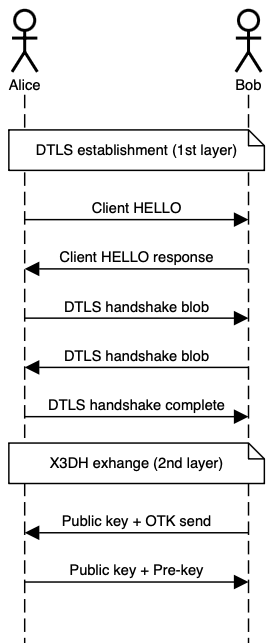
\includegraphics[scale=0.4]{./authentification/diagram.png}
    \caption{Diagram of exchanges before the the first message.}
\end{figure}

\section{Datagram Transport Layer Security}
\label{sec:dtls}

Datagram Transport Layer Security (DTLS) is a protocol based on TLS, designed 
to prevent eavesdropping, tampering, and message forgery \cite{rfc9147}. It 
guarantees a reliable and in-order delivery of data, unlike datagram transport. 
DLTS is the first security layer of the Turms protocol. You MUST implement a 
first security layer, ensuring encryption, authenticity and integrity.
\bigskip

See: \href{https://datatracker.ietf.org/doc/rfc9147/}{RFC 9147}.

\section{Extended Triple Diffie-Hellman}

In P2P, there is no trusted server to guarantee that Alice and Bob's public 
keys are correct. The security layer provided by DTLS ensures that the keys 
have not been altered by a third party (MITM).
\bigskip

If Alice initiated the WebRTC connection, then Bob initiates the key exchange. 
Bob, as initiator, send to Alice its public key and one-time key \((IK_B, 
OPK_B)\).

\begin{align*}
    DH_1 &= DH(IK_B, SPK_A)\\
    DH_2 &= DH(EK_B, IK_A)\\
    DH_3 &= DH(EK_B, SPK_A)\\
    DH_4 &= DH(EK_B, OPK_A)\\
    SK &= \mathrm{KDF}_{\text{Concat}}\left( DH_1 \,\|\, DH_2 \,\|\, DH_3 
\,\|\, DH_4 \right)
\end{align*}

with \(\mathrm{KDF}\) a key derivation function, often based on HKDF with 
SHA-256.

\begin{align*}
    (\text{RootKey}, \text{ChainKey}) &= \mathrm{KDF}_{\text{Root}}(SK)\\
    \text{MessageKey} &= \mathrm{KDF}_{\text{Chain}}(\text{ChainKey})
\end{align*}

Bob checks Alice's pre-signed \(SPK_A\) is authentic:

\begin{equation*}
    \mathrm{VerifySig}(IK_A, \mathrm{Sig}_{IK_A}(SPK_A)) = 1
\end{equation*}

As described on Signal's specification, \enquote{the parties may compare their 
identity public keys \(IK_A\) and \(IK_B\) through some authenticated 
channel}\cite[p. 7]{marlinspike2016}. Turms has chosen to ensure P2P security 
by conducting exchanges over the secure DTLS channel. You MUST implement DTLS 
connection before exchange public keys. This choice mitigate subsections 4.1, 
4.7 and 4.8 of X3DH protocol \enquote{Security 
considerations}\cite{marlinspike2016}, but creates possible non-deniability of 
communication between peers.

\section{Double Ratchet}

The Double Ratchet protocol extends X3DH by ensuring \enquote{Perfect Forward 
Secrecy} and \enquote{Post-Compromise Security}\cite{perrin2025}. It combines
two key update mechanisms:
\begin{itemize}
    \item one Diffie-Hellman key ratchet (asymmetric);
    \item un symmetrical ratchet (based on a KDF).
\end{itemize}

After the X3DH exchange, both parties have the same initial root key:

\[
    RK_0 = \text{KDF}_{\text{Root}}(SK_{\text{X3DH}})
\]

Each party also has a pair of initial Diffie-Hellman keys:

\[
    (DH_s^{(0)}, DH_r^{(0)})
\]

Each time a new public key \(DH_r^{(t)}\) is received from the other party:
\begin{align*}
    DH_{\text{out}}^{(t)} &= DH(DH_s^{(t-1)}, DH_r^{(t)}) \\
    RK_t, CK_r^{(t)} &= \mathrm{KDF}_{\text{Root}}(RK_{t-1}, 
DH_{\text{out}}^{(t)}) \\
    DH_s^{(t)} &\leftarrow \text{GenerateKeyPair()} \\
    RK_t, CK_s^{(t)} &= \mathrm{KDF}_{\text{Root}}(RK_t, DH(DH_s^{(t)}, 
DH_r^{(t)}))
\end{align*}

Thus, with each Diffie-Hellman jump, the root key and the two strings 
(send/receive) are renewed. For each message sent, the send string is derived:

\[
    CK_s^{(i+1)}, MK_s^{(i)} = \mathrm{KDF}_{\text{Chain}}(CK_s^{(i)})
\]

For each message received:

\[
    CK_r^{(j+1)}, MK_r^{(j)} = \mathrm{KDF}_{\text{Chain}}(CK_r^{(j)})
\]

\begin{align*}
    \mathrm{Encrypt}(MK_s^{(i)}, &\text{plaintext}) \to \text{ciphertext}\\
    \mathrm{Decrypt}(MK_r^{(j)}, &\text{ciphertext}) \to \text{plaintext}
\end{align*}

A message key MUST NEVER be reused, to ensure perfect confidentiality of old 
messages even in the event of future compromise.

\begin{align*}
    RK_0 &= \mathrm{KDF}_{\text{Root}}(SK_{\text{X3DH}}) \\[6pt]
    RK_t, CK_r^{(t)} &= \mathrm{KDF}_{\text{Root}}\big(RK_{t-1}, 
DH(DH_s^{(t-1)}, DH_r^{(t)})\big) \\[6pt]
    RK_t, CK_s^{(t)} &= \mathrm{KDF}_{\text{Root}}\big(RK_t, DH(DH_s^{(t)}, 
DH_r^{(t)})\big) \\[6pt]
    CK_{x}^{(i+1)}, MK_{x}^{(i)} &= \mathrm{KDF}_{\text{Chain}}(CK_{x}^{(i)}), 
\quad x \in \{s, r\}
\end{align*}

\begin{itemize}
    \item \textbf{Perfect Forward Secrecy}: compromising a future key does not 
        reveal previous messages.
    \item \textbf{Post-Compromise Security}: after a DH jump, the new keys 
        become secure again.
    \item \textbf{Unidirectional derivation}: no derived key can be traced back 
        to the root key.
\end{itemize}

\chapter{Messages}

\section{Network}

\subsection{Transport}

\[
\text{WebRTCManager} = 
\left(
\begin{array}{l}
\text{peer\_connection} \in \mathcal{P},\\
\text{ice} \subseteq \mathcal{I},\\
\text{channel} \in \mathcal{C} \cup \{\emptyset\},\\
\text{is\_initiator} \in \{\text{false}, \text{true}\},\\
\text{offer} \in \Sigma^*
\end{array}
\right)
\]

\subsection{Fallback}

\section{Events}

\begin{center}
\begin{tikzpicture}
\begin{umlpackage}[type=peer-to-peer]{ChatModel}

\umlenum[x=0,y=0]{Event}{
    + DHKey(x3dh: X3DH) \\
    + Message(msg: Message) \\
    + Typing()
}{}

\umlclass[x=-6,y=-4]{X3DH}{
    + public\_key : Vector<Byte> \\
    + otk : Vector<Byte>
}{}

\umlclass[x=0,y=-8]{Message}{
    + author : String \\
    + recipient : String \\
    + content : String \\
    + timestamp : DateTime \\
    + edited\_timestamp : DateTime \\
    + reactions : Vector<Char> \\
    + attachments : Vector<Attachment> \\
    + flags : Flags
}{}

\umlclass[x=6,y=-8]{Attachment}{
    + filename : String \\
    + mime\_type : Optional<String> \\
    + url : Optional<String> \\
    + blob : Optional<Vector<Byte>> \\
    + flags : Flags
}{}

\umlclass[x=0,y=-12]{Flags}{
    + URGENT : Boolean \\
    + EPHEMERAL : Boolean
}{}

\umlaggreg[arg=hasX3DH, mult=1, pos=0.5]{Event}{X3DH}
\umlaggreg[arg=hasMessage, mult=1, pos=0.5]{Event}{Message}
\umlaggreg[arg=hasAttachments, mult=*, pos=0.5]{Message}{Attachment}
\umlaggreg[arg=usesFlags, mult=1, pos=0.5]{Message}{Flags}
\umlaggreg[arg=usesFlags, mult=1, pos=0.5]{Attachment}{Flags}
\end{umlpackage}
\end{tikzpicture}
\end{center}

\section{Content}

\section{Cryptography}

\chapter{Discovery server}
\label{chap:discovery}

\section{Decentralized authentification}

\section{Message buffering}

\printbibliography

\clearpage
\appendix

\begin{appendices}
\addcontentsline{toc}{chapter}{Démonstration de la résilience d'un réseau P2P}
\includepdf[pages={-},
            pagecommand={\thispagestyle{plain}}
           ]{appendices/resilience.pdf}
\end{appendices}

\end{document}
